\documentclass{standalone}

\usepackage{lscape}
%Math typesetting packages
\usepackage{amsfonts, amssymb, amsmath, latexsym, amsthm,xparse, bm}
\newcommand\simiid{\stackrel{iid}{\sim}}
\newcommand\simind{\stackrel{ind}{\sim}}
\NewDocumentCommand{\qfrac}{smm}{%
  \dfrac{\IfBooleanT{#1}{\vphantom{\big|}}#2}{\mathstrut #3}%
}

\usepackage{tikz}
\usetikzlibrary{calc,arrows,positioning,shapes,shapes.gates.logic.US,trees, intersections}

\begin{document}

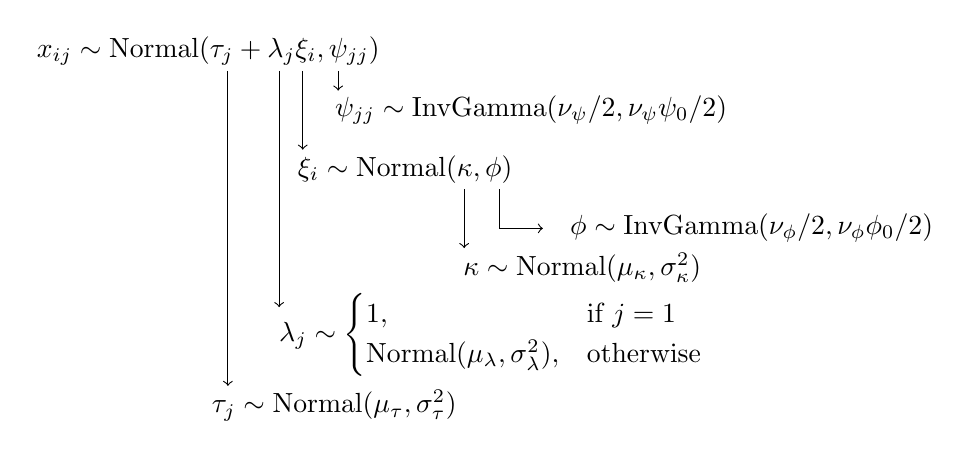
\begin{tikzpicture}
  \node at (0,0) {$x_{ij} \sim \mathrm{Normal}(\tau_j + \lambda_j\xi_i, \psi_{jj})$} ;
  	\draw[->] (1.65, -0.25) -- (1.65, -0.5);
  	\node at (4.1, -0.75) {$\psi_{jj}\sim \mathrm{InvGamma}(\nu_{\psi}/2, \nu_{\psi}\psi_0/2)$};
  		%\draw[->] (6, -1) |- (6.3, -1.25);
  		%\node at (7, -1.25) {$\psi_0 = 2$};
  		%\draw[->] (4.6, -1) -- (4.6, -1.25);
  		%\node at (5.15, -1.5) {$\nu_{\psi} = 10$};
  	\draw[->] (1.2,-0.25) -- (1.2,-1.25);
  	\node at (2.5, -1.5) {$\xi_i \sim \mathrm{Normal}(\kappa,\phi)$};
  		\draw[->] (3.7, -1.75) |- (4.25, -2.25);
  		\node at (6.9, -2.25) {$\phi\sim \mathrm{InvGamma}(\nu_{\phi}/2, \nu_{\phi}\phi_0/2)$};
  		\draw[->] (3.25, -1.75) -- (3.25, -2.5);
	  	\node at (4.75, -2.75) {$\kappa \sim \mathrm{Normal}(\mu_{\kappa},\sigma^2_{\kappa})$};
	  	
	\draw[->] (0.9,-0.25) -- (0.9,-3.25);
  	\node at (3.6, -3.6) {$\lambda_j \sim \begin{cases} 1, & \text{if}\ j=1 \\ \mathrm{Normal}(\mu_{\lambda}, \sigma^2_{\lambda}), & \text{otherwise} \end{cases}$};
  	\draw[->] (0.25, -0.25) -- (0.25, -4.25);
  	\node at (1.6, -4.5) {$\tau_j \sim \mathrm{Normal}(\mu_{\tau},\sigma^2_{\tau})$};
  		
\end{tikzpicture}

\end{document}